\chapter{Cables}\index{cables}

Es tracten en aquest cap\'{\i}tol q\"{u}estions relatives als cables el\`{e}ctrics.

\section{Resist\`{e}ncia}\index{cables!resist\`{e}ncia}

\subsection{Resist\`{e}ncia d'un conductor}

La resist\`{e}ncia $R$ d'un conductor dep\`{e}n de la resistivitat $\rho$
del material, de la llargada $l$ del conductor i de la seva secci\'{o}
$S$.
\begin{equation}
   R= \rho \frac{l}{S}
\end{equation}
\index{$\rho$}

\index{resistivitat!variaci\'{o} amb la temperatura}La resistivitat no
\'{e}s un valor constant sin\'{o} que dep\`{e}n de la temperatura, a major
temperatura major resistivitat. Coneixent la resistivitat $\rho_1$ a una
temperatura $T_1$ es pot calcular la resistivitat $\rho_2$ a una altra
temperatura $T_2$, a partir del coeficient de variaci\'{o} de la
resistivitat amb la temperatura $\alpha_1$ donat a la temperatura $T_1$.
\begin{equation}
   \rho_2 = \rho_1 [1 + \alpha_1 (T_2 - T_1)]\label{eq:resistivitat}
\end{equation}
\index{$\alpha$}

\index{resistivitat!valors}En la Taula
\vref{taula:param-elc} es donen valors de la resistivitat i dels
coeficients de variaci\'{o} de la resistivitat amb la temperatura a
\SI{20}{\celsius} i a \SI{0}{\celsius}, per a diversos materials.
\begin{table}[htb]
   \caption{\label{taula:param-elc} Par\`{a}metres el\`{e}ctrics d'alguns materials}
   \[ \begin{array}{lccc}
   \toprule[1pt]
   \text{Material} & \rho_{\SI{20}{\celsius}}\,[\si{\ohm.mm^2/m}] & \alpha_{\SI{20}{\celsius}}\,[\si{\celsius^{-1}}] &
   \alpha_{\SI{0}{\celsius}}\,[\si{\celsius^{-1}}]
   \\
   \midrule
      \text{Alumini} & \num{0,02825} & \num{0,00391} & \num{0,00424} \\
      \text{Coure}   & \num{0,01723} & \num{0,00393} & \num{0,00427} \\
      \text{Plata}   & \num{0,01645} & \num{0,00380} & \num{0,00412} \\
   \bottomrule[1pt]
   \end{array}   \]
\end{table}

La resist\`{e}ncia aix\'{\i} calculada \'{e}s v\`{a}lida quan el corrent que circula
pel cable \'{e}s corrent continu.

Quan el corrent que circula pel cable \'{e}s
corrent altern cal tenir en compte l'efecte pe{\l.l}icular, el qual
li provoca un augment de la resist\`{e}ncia, causat perqu\`{e} el corrent
tendeix a circular m\'{e}s per la zona perif\`{e}rica del conductor que per
la zona central; l'efecte \'{e}s important per a valors elevats de la
secci\'{o} del conductor o de la freq\"{u}\`{e}ncia del corrent.\index{efecte pe{\l.l}icular}

\index{resist\`{e}ncia!efectiva}La resist\`{e}ncia efectiva es troba a
partir de la resist\`{e}ncia calculada anteriorment per a corrent
continu, i d'un factor k que t\'{e} en compte l'efecte pe{\l.l}icular.
\begin{equation}
   R\ped{efectiva} = \text{k} R
\end{equation}

En la Taula \vref{taula:const_r_ef} es donen valors\footnote{Valors obtinguts del llibre {"<}Teor\'{\i}a de Circuitos. Fundamentos, 3\textordfeminine\ edici\'{o}n{">}, Enrique Ras, Marcombo Boixareu Editores (p\`{a}g. 114).} de k per a conductors de coure i d'alumini, per a diversos valors del producte de la secci\'{o} del conductor per la freq\"{u}\`{e}ncia del corrent.
\begin{table}[htb]
   \caption{\label{taula:const_r_ef} Valors de k pel c\`{a}lcul de la resist\`{e}ncia efectiva}
   \begin{center}\begin{tabular}{r<{\hspace{2.5em}}>{\hspace{3.5em}}cc}
   \toprule[1pt]
   %\renewcommand*{\multirowsetup}{\centering}
   \multirow{2}{25mm}{\rule{0mm}{4.5mm}Secci\'{o}$\,\times\,$Freq\"{u}\`{e}ncia\\{}\rule{8mm}{0mm}[\si{mm^2.Hz}]} & \multicolumn{2}{c}{k, segons el material del conductor} \\ \cmidrule(rl){2-3}
    & Cu & Al \\
   \midrule
  \num[group-minimum-digits = 4]{5000} &  \num{1,000} & \num{1,000} \\
  \num{10000} & \num{1,008} & \num{1,000} \\
  \num{15000} & \num{1,025} & \num{1,006} \\
  \num{20000} & \num{1,045} & \num{1,015} \\
  \num{25000} & \num{1,070} & \num{1,026} \\
  \num{30000} & \num{1,096} & \num{1,040} \\
  \num{35000} & \num{1,126} & \num{1,053} \\
  \num{40000} & \num{1,158} & \num{1,069} \\
  \num{45000} & \num{1,195} & \num{1,085} \\
  \num{50000} & \num{1,230} & \num{1,104} \\
  \num{75000} & \num{1,433} & \num{1,206} \\
  \num{100000} & \num{1,622} & \num{1,330} \\
   \bottomrule[1pt]
   \end{tabular} \end{center}
\end{table}

\subsection{Resist\`{e}ncia d'un cable}

La resist\`{e}ncia d'un cable $R\ped{Cable}$ dep\`{e}n del nombre de conductors per fase $n$ (o
per pol, en corrent continu), de la resist\`{e}ncia de cada conductor $R\ped{Conductor}$ i del
tipus de tensi\'{o} el\`{e}ctrica a la qual estigui sotm\`{e}s el cable (monof\`{a}sica, trif\`{a}sica,
cont\'{\i}nua, etc.).

\subsubsection*{Corrent continu o altern monof\`{a}sic}
\begin{equation}\label{eq:r_cc_mono}
    R\ped{Cable} = 2\, \frac{R\ped{Conductor}}{n}
\end{equation}

El valor multiplicatiu 2, prov\'{e} del fet que cal tenir en compte tant el conductor d'anada
com el de tornada.

\subsubsection*{Corrent altern trif\`{a}sic equilibrat}
\vspace{-5mm}
\begin{equation}\label{eq:r_trifas}
R\ped{Cable} = \frac{R\ped{Conductor\;fase}}{n}
\end{equation}

At\`{e}s que no circula corrent pel neutre, la seva resist\`{e}ncia no hi t\'{e} cap influ\`{e}ncia.

\subsubsection*{Corrent altern trif\`{a}sic desequilibrat}
\begin{equation}
    R\ped{Cable\;fase} = \frac{R\ped{Conductor\;fase}}{n\ped{fase}} \qquad\qquad
    R\ped{Cable\; neutre} = \frac{R\ped{Conductor\;neutre}}{n\ped{neutre}}
\end{equation}

En aquest cas cal tenir en compte que els corrents que circulen per les fase i pel neutre
s\'{o}n diferents.


\section{Caiguda de tensi\'{o}}\index{cables!caiguda de tensi\'{o}}

La caiguda de tensi\'{o} $\Delta U$ en un cable es defineix com la difer\`{e}ncia entre els m\`{o}duls de les tensions a l'origen $|{\cmplx{U}\ped{O}}|$ i al final $|\cmplx{U}\ped{F}|$ del cable.
\begin{equation}
   \Delta U \equiv |\cmplx{U}\ped{O}| - |\cmplx{U}\ped{F}|
\end{equation}

\subsection{Caiguda de tensi\'{o} en corrent continu}\index{cables!caiguda de tensi\'{o}!en corrent continu}

En corrent continu la caiguda de tensi\'{o} dep\`{e}n del corrent $I$ que circula pel cable i de la  resist\`{e}ncia del propi cable, calculada segons l'equaci\'{o} \eqref{eq:r_cc_mono}.
\begin{equation}
   \Delta U = I R\ped{Cable}
\end{equation}

\subsection{Caiguda de tensi\'{o} en corrent altern}\index{cables!caiguda de tensi\'{o}!en corrent altern}

\index{factor!de pot\`{e}ncia}En corrent altern la caiguda de tensi\'{o}
dep\`{e}n del  corrent $\cmplx{I}$ que circula pel cable, de la
resist\`{e}ncia i la react\`{a}ncia del propi cable i del factor de
pot\`{e}ncia $\cos \varphi$. El diagrama fasorial d'aquestes magnituds
es pot veure en la Figura \vref{pic:cdt_ca}.
\begin{figure}[htb]
   \centering
   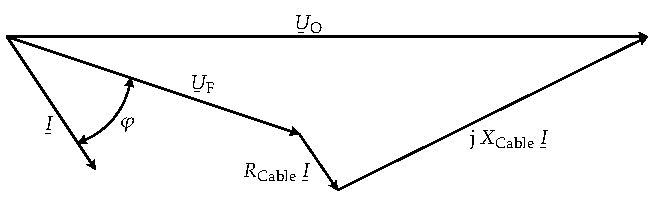
\includegraphics{Imatges/Cap-Cables-Caiguda-Tensio.pdf}
   \caption{Caiguda de tensi\'{o} en corrent altern}\label{pic:cdt_ca}
\end{figure}

Quan es tracta de corrent monof\`{a}sic, la resist\`{e}ncia del cable es calcula segons l'equaci\'{o}
\eqref{eq:r_cc_mono}; la react\`{a}ncia del cable $X\ped{Cable}$ es calcula de forma an\`{a}loga
amb la mateixa equaci\'{o}, a partir de la react\`{a}ncia dels conductors $X\ped{Conductor}$.

Pel que fa al corrent trif\`{a}sic, se suposa equilibrat, i per tant s'utilitza l'equaci\'{o}
\eqref{eq:r_trifas} per calcular la resist\`{e}ncia del cable $R\ped{Cable}$ (i de forma
an\`{a}loga la react\`{a}ncia $X\ped{Cable}$). Addicionalment, els corrents fan refer\`{e}ncia als
corrents de fase i les tensions a les tensions fase--neutre; l'angle $\varphi$ \'{e}s per
tant l'angle entre la tensi\'{o} final fase--neutre i el corrent de fase.

Disposem en aquest cas de dues equacions, una d'exacta i una altre d'aproximada (per a valors elevats de $\cos \varphi$).
\begin{subequations}
\begin{align}
   \Delta U &= |\cmplx{I}| \,( R\ped{Cable} \cos \varphi + X\ped{Cable} \sin \varphi) + |\cmplx{U}\ped{O}| - \sqrt{|\cmplx{U}\ped{O}|^2 - |\cmplx{I}|^2 ( X\ped{Cable} \cos \varphi - R\ped{Cable} \sin \varphi )^2} \label{eq:cdt_trif_exact} \\
   \Delta U &\approx |\cmplx{I}| \,( R\ped{Cable} \cos \varphi + X\ped{Cable} \sin \varphi) \qquad \text{si} \; \cos \varphi \gtrapprox \num{0,8} \label{eq:cdt_trif_aprox}
\end{align}
\end{subequations}

\vspace{2mm}
\begin{exemple}
   Es tracta de calcular la caiguda de tensi\'{o} en un sistema trif\`{a}sic on $|\cmplx{U}\ped{O}| = \SI{380}{V}$ (fase--fase), $|\cmplx{I}|=\SI{630}{A}$ i $\cos \varphi = \num{0,87}$(i). La uni\'{o} entre els extrems origen  i final est\`{a} formada per tres cables en para{\l.l}el de $\SI{240}{mm^2}$ de secci\'{o} cadascun i $\SI{400}{m}$ de llargada; els valors per fase de resist\`{e}ncia i induct\`{a}ncia s\'{o}n $\SI{0,095}{\ohm/km}$ i $\SI{0,102}{\ohm/km}$ respectivament.

A partir de l'equaci\'{o} \eqref{eq:r_trifas} calculem els valors de $R\ped{Cable}$ i de $X\ped{Cable}$.
\[
   R\ped{Cable} = \frac{\SI{0,095}{\ohm/km}\times \SI{0,4}{km}}{3} = \SI{0,0127}{\ohm}
\]
\[
   X\ped{Cable} = \frac{\SI{0,102}{\ohm/km}\times \SI{0,4}{km}}{3} = \SI{0,0136}{\ohm}
\]

Obtenim a continuaci\'{o} el valor de $\sin \varphi$:
\[
   \sin \varphi = \sqrt{1-\num{0,87}^2} = \num{0,49}
\]

Calculem en primer lloc la caiguda de tensi\'{o} de forma aproximada utilitzant l'equaci\'{o} \eqref{eq:cdt_trif_aprox}.
\[
   \Delta U \approx \SI{630}{A} \times ( \SI{0,0127}{\ohm} \times \num{0,87} + \SI{0,0136}{\ohm} \times \num{0,49} ) = \SI{11,16}{V}
\]

que en tant per cent respecte la tensi\'{o} a l'origen representa:
$\frac{\SI{11,16}{V}}{380/\sqrt{3}\unit{V}} \times 100 = \SI{5,09}{\%} $

Finalment, calculem la caiguda de tensi\'{o} exacta utilitzant l'equaci\'{o} \eqref{eq:cdt_trif_exact}.
\[ \begin{split}
   \Delta U &=  \SI{630}{A} \times( \SI{0,0127}{\ohm} \times \num{0,87} + \SI{0,0136}{\ohm} \times \num{0,49}) + \frac{380}{\sqrt{3}}\unit{V} \,- \\
    & \quad - \sqrt{\left(380/\sqrt{3}\unit{V}\right)^2 - \left(\SI{630}{A}\right)^2 \times  \left( \SI{0,0136}{\ohm} \times \num{0,87} - \SI{0,0127}{\ohm} \times \num{0,49} \right)^2 } \,= \SI{11,19}{V}
\end{split} \]

que en tant per cent respecte la tensi\'{o} a l'origen representa:
$\frac{\SI{11,19}{V}}{380/\sqrt{3}\unit{V}} \times 100 = \SI{5,10}{\%} $
\end{exemple}

\section{Capacitat t\`{e}rmica en curt circuit}\index{cables!capacitat t\`{e}rmica en curt circuit}

Quan hi ha un curt circuit en un cable, tot el calor generat no es transmet a l'exterior en els instants inicials, sin\'{o} que s'acumula en la massa del conductor, incrementant la seva temperatura (proc\'{e}s adiab\`{a}tic). En aquestes condicions es pot aplicar l'equaci\'{o}:
\begin{equation}\label{eq:Icc_termica}
   I\ped{cc} = S\, \frac{\text{C}}{\sqrt{t}} \quad
   \begin{cases}
   I\ped{cc} &:\; \text{expressat en\unit{A}} \\
   S         &:\; \text{expressat en\unit{mm^2}} \\
   t         &:\; \text{expressat en\unit{s}} \\
   \text{C}  &:\; \text{par\`{a}metre dependent del tipus de cable}
   \end{cases}
\end{equation}

$I\ped{cc}$ \'{e}s la intensitat de curt circuit que circula pel conductor, $S$ \'{e}s la secci\'{o} del conductor, $t$ \'{e}s el temps m\`{a}xim que pot durar el curt circuit sense que es malmeti el cable, i C \'{e}s un par\`{a}metre que dep\`{e}n del material  del conductor i del seu a\"{\i}llament. En la Taula \vref{taula:const_termica} es donen valors\footnote{Valors obtinguts del cat\`{a}leg del fabricant {"<}General Cable{">}.} de C per a diferents materials del conductor i de l'a\"{\i}llament.
\begin{table}[htb]
   \caption{\label{taula:const_termica} Valors de C pel c\`{a}lcul de curt circuits en cables}
   \begin{center}\begin{tabular}{c>{\hspace{2.5em}}cc}
   \toprule[1pt]
   \renewcommand*{\multirowsetup}{\centering}
   \multirow{2}{25mm}{\rule{0mm}{4mm}Material del\\conductor} & \multicolumn{2}{c}{C, segons el material de l'a\"{\i}llament} \\ \cmidrule(rl){2-3}
    & PVC & EPR i XLPE \\
   \midrule
   Cu & 115 & 142 \\
   Al & 75 & 93 \\
   \bottomrule[1pt]
   \end{tabular} \end{center}
\end{table}

\begin{exemple}
   Es tracta de calcular el temps m\`{a}xim durant el qual un cable de coure de $\SI{50}{mm^2}$ amb a\"{\i}llament d'EPR, pot suportar un corrent de curt circuit de $\SI{15}{kA}$.

A partir de l'equaci\'{o} \eqref{eq:Icc_termica} calculem el temps m\`{a}xim demanat:
\[
   t = \left( \frac{S\,C}{I\ped{cc}} \right) ^2 = \left( \frac{\SI{50}{mm^2}\times 142}{\SI{15000}{A}} \right) ^2 = \SI{224}{ms}
\]
\end{exemple}

\section{Conversi\'{o} entre unitats americanes i unitats SI}

\subsection{{"<}Mils{">} (mil), {"<}circular mils{">} (cmil o CM) i {"<}thousand circular mils{">} (kcmil o MCM)}\label{sec:MCM}
\index{mil}\index{cmil}\index{CM}\index{kcmil}\index{MCM}
\index{mils@\guillemotleft mils\guillemotright} \index{circular mils@\guillemotleft circular mils\guillemotright} \index{thousand circular mils@\guillemotleft thousand circular mils\guillemotright}

\index{mils@\guillemotleft mils\guillemotright!difinici\'{o}} \index{circular mils@\guillemotleft circular mils\guillemotright!difinici\'{o}} \index{thousand circular mils@\guillemotleft thousand circular mils\guillemotright!difinici\'{o}}Les definicions d'aquestes tres unitats utilitzades en la mesura de di\`{a}metres i seccions de cables s\'{o}n:
\begin{align}
  \SI{1}{mil} &\equiv \text{Una mi{\l.l}\`{e}sima de polsada} \\
  \SI{1}{cmil} = \SI{1}{CM} &\equiv  \text{\`{A}rea d'un cercle de di\`{a}metre igual a \SI{1}{mil}} \\
  \SI{1}{kcmil} = \SI{1}{MCM} &\equiv \SI{1000}{cmil} = \SI{1000}{CM}
\end{align}

\index{mils@\guillemotleft mils\guillemotright!equival\`{e}ncies} \index{circular mils@\guillemotleft circular mils\guillemotright!equival\`{e}ncies} \index{thousand circular mils@\guillemotleft thousand circular mils\guillemotright!equival\`{e}ncies}Es donen a continuaci\'{o} algunes conversions d'aquestes unitats:
\begin{align}
   \SI{1}{mil} &= \SI{e-3}{in}  \\
  \SI{1}{mil} &= \SI{e-3}{in} \times \frac{\SI{25,4}{mm}}{\SI{1}{in}} = \SI{25,4e-3}{mm}  \\
  \SI{1}{cmil} &= \frac{\piup}{4}\unit{mil^2} = \SI{0,785398}{mil^2}   \\
   \SI{1}{cmil} &= \frac{\piup}{4}\times \SI{e-6}{in^2} = \SI{0,785398e-6}{in^2} \\
   \SI{1}{cmil} &= \frac{\piup}{4} \times \SI{e-6}{in^2} \times \frac{\SI{645,16}{mm^2}}{\SI{1}{in^2}} = \SI{506,7075e-6}{mm^2}
   \\[1ex]
   \SI{1}{kcmil} &= \SI{785,398}{mil^2}  = \SI{0,785398e-3}{in^2} = \SI{0,5067075}{mm^2}
\end{align}

Una relaci\'{o} \'{u}til entre di\`{a}metres  i seccions \'{e}s la seg\"{u}ent: la secci\'{o} $S$ d'un cercle expressada en {"<}circular mils{">} \'{e}s igual al quadrat del di\`{a}metre $d$ del cercle expressat en {"<}mils{">}.
\begin{equation}
   S = d^2 \quad
   \begin{cases}
   S &:\; \text{expressat en\unit{cmil}} \\
   d &:\; \text{expressat en\unit{mil}}
   \end{cases}
\end{equation}

En la Taula \vref{taula:MCM} es relacionen els di\`{a}metres i seccions en diverses unitats, dels conductors usualment disponibles compresos entre $\SI{2000}{kcmil}$ i $\SI{250}{kcmil}$.
\begin{longtable}{r<{\hspace{0.6em}}rrrrr}
\caption{\label{taula:MCM}Dimensions de cables definits en kcmil} \\
\toprule[1pt]
    \multicolumn{3}{c}{Secci\'{o}} &   \multicolumn{3}{c}{Di\`{a}metre}         \\
    \cmidrule(rl){1-3} \cmidrule(rl){4-6}
    \multicolumn{1}{c}{[kcmil]}  &    \multicolumn{1}{c}{[\si{in^2}]}  & \multicolumn{1}{c}{[\si{mm^2}]}  & \multicolumn{1}{c}{[mil]}
           &    \multicolumn{1}{c}{[in]} &   \multicolumn{1}{c}{[mm]}   \\
\midrule \endfirsthead
\caption[]{(\emph{ve de la p\`{a}gina anterior})} \\
\toprule[1pt]
    \multicolumn{3}{c}{Secci\'{o}} &   \multicolumn{3}{c}{Di\`{a}metre}         \\
    \cmidrule(rl){1-3} \cmidrule(rl){4-6}
    \multicolumn{1}{c}{[kcmil]}  &    \multicolumn{1}{c}{[\si{in^2}]}  & \multicolumn{1}{c}{[\si{mm^2}]}  & \multicolumn{1}{c}{[mil]}
           &    \multicolumn{1}{c}{[in]} &   \multicolumn{1}{c}{[mm]}   \\
\midrule \endhead
\midrule
\multicolumn{6}{r}{(\emph{continua a la p\`{a}gina seg\"{u}ent})}
\endfoot
\endlastfoot
2000 &   \num{1,570796} &   \num{1013,4150} & \num{1414,21356} &  \num{1,4142136} &   \num{35,92102} \\
1750 &   \num{1,374447} &   \num{886,7381}  & \num{1322,87566} &  \num{1,3228757} &   \num{33,60104} \\
1600 &   \num{1,256637} &   \num{810,7320}  & \num{1264,91106} &  \num{1,2649111} &   \num{32,12874} \\
1500 &   \num{1,178097} &   \num{760,0612}  & \num{1224,74487} &  \num{1,2247449} &   \num{31,10852} \\
1250 &   \num{0,981748} &   \num{633,3843}  & \num{1118,03399} &  \num{1,1180340} &   \num{28,39806} \\
1000 &   \num{0,785398} &   \num{506,7075}  & \num{1000,00000} &  \num{1,0000000} &   \num{25,40000} \\
 800 &   \num{0,628319} &   \num{405,3660}  & \num{ 894,42719} &  \num{0,8944272} &   \num{22,71845} \\
 750 &   \num{0,589049} &   \num{380,0306}  & \num{ 866,02540} &  \num{0,8660254} &   \num{21,99705} \\
 700 &   \num{0,549779} &   \num{354,6952}  & \num{ 836,66003} &  \num{0,8366600} &   \num{21,25116} \\
 600 &   \num{0,471239} &   \num{304,0245}  & \num{ 774,59667} &  \num{0,7745967} &   \num{19,67476} \\
 500 &   \num{0,392699} &   \num{253,3537}  & \num{ 707,10678} &  \num{0,7071068} &   \num{17,96051} \\
 450 &   \num{0,353429} &   \num{228,0184}  & \num{ 670,82039} &  \num{0,6708204} &   \num{17,03884} \\
 400 &   \num{0,314159} &   \num{202,6830}  & \num{ 632,45553} &  \num{0,6324555} &   \num{16,06437} \\
 350 &   \num{0,274889} &   \num{177,3476}  & \num{ 591,60798} &  \num{0,5916080} &   \num{15,02684} \\
 300 &   \num{0,235619} &   \num{152,0122}  & \num{ 547,72256} &  \num{0,5477226} &   \num{13,91215} \\
 250 &   \num{0,196350} &   \num{126,6769}  & \num{ 500,00000} &  \num{0,5000000} &   \num{12,70000} \\
\bottomrule[1pt]
\end{longtable}

D'aquesta taula es pot veure que: $\text{Secci\'{o} en}\unit{mm^2} \approx \dfrac{\text{Secci\'{o} en}\unit{kcmil}}{2}$.

\break
\subsection{{"<}American Wire Gauge{">} (AWG)}
\index{AWG (\guillemotleft American Wire Gauge\guillemotright)}

\index{AWG (\guillemotleft American Wire Gauge\guillemotright)!definici\'{o}}L'{"<}American Wire Gauge{">}, anomenat tamb\'{e} {"<}Brown \& Sharp Gauge{">}, \'{e}s un sistema de numeraci\'{o} de conductors de coure segons el seu di\`{a}metre. A cada n\'{u}mero AWG correspon un valor de di\`{a}metre; els successius di\`{a}metres formen una progressi\'{o} geom\`{e}trica descendent (en augmentar el n\'{u}mero AWG, disminueix el di\`{a}metre).

La ra\'{o} d'aquesta progressi\'{o} geom\`{e}trica s'obt\'{e} de la seg\"{u}ent consideraci\'{o}: hi ha dos valors de refer\`{e}ncia, AWG 36, el qual t\'{e} assignat un di\`{a}metre de \SI{5}{mil}, i AWG 4/0 (tamb\'{e} anomenat AWG 0000), el qual t\'{e} assignat un di\`{a}metre de \SI{460}{mil}. Entre aquest dos valors de refer\`{e}ncia hi ha una diferencia de 39 unitats (vegeu la Taula \vref{taula:AWG}), i per tant, sent $r\ped{d}$ la ra\'{o} de di\`{a}metres buscada, tenim:
\begin{equation}
   \SI{5}{mil} = \SI{460}{mil} \times r\ped{d}^{39} \quad \rightarrow \quad r\ped{d} = \left( \frac{\SI{5}{mil}}{\SI{460}{mil}} \right)^{1/39} = \left( \frac{1}{92} \right)^{1/39} = 92^{-1/39}
\end{equation}

En ser la secci\'{o} d'un conductor proporcional al quadrat del seu di\`{a}metre, les seccions dels successius n\'{u}meros AWG formen una progressi\'{o} geom\`{e}trica  descendent de ra\'{o} $r\ped{S}$ igual a: \begin{equation}
   r\ped{S} = r\ped{d}^2 = 92^{-2/39}
\end{equation}

Finalment, en ser la resist\`{e}ncia d'un conductor inversament proporcional a la seva secci\'{o}, les resist\`{e}ncies dels successius n\'{u}meros AWG formen una progressi\'{o} geom\`{e}trica ascendent de ra\'{o} $r\ped{R}$ igual a:
\begin{equation}
   r\ped{R} = \frac{1}{r\ped{S}} = 92^{2/39}
\end{equation}

A partir d'aquestes raons, i coneixent el di\`{a}metre $d$, la secci\'{o} $S$ i la resist\`{e}ncia $R$ d'un n\'{u}mero AWG $n$, podem calcular aquests par\`{a}metres per a un altre n\'{u}mero AWG, $k$ unitats posterior o $k$ unitats anterior:

\begin{equation}
   \begin{array}{rllllll}
     \text{AWG:}         & & n & & n+k                & & n-k \\
     \text{Di\`{a}metre:}    & & d & & d\times 92^{-k/39}  & & d\times 92^{k/39} \\
     \text{Secci\'{o}:}      & & S & & S\times 92^{-2k/39} & & S\times 92^{2k/39} \\
     \text{Resist\`{e}ncia:} & & R & & R\times 92^{2k/39}  & & R\times 92^{-2k/39}
   \end{array}
\end{equation}

Per a alguns valors particulars de $k$ es compleixen de forma aproximada les seg\"{u}ents relacions:

\begin{list}{}
   {\setlength{\labelwidth}{15mm} \setlength{\leftmargin}{17mm} \setlength{\labelsep}{2mm}}

   \item[$k=6$\hfill] En augmentar en 6  unitats el n\'{u}mero AWG, el di\`{a}metre es divideix per 2
                 $(92^{-6/39}\approx \num{0,5})$.

   \item[$k=-6$\hfill] En disminuir en 6 unitats el n\'{u}mero AWG, el di\`{a}metre es multiplica per 2
                 $(92^{6/39}\approx 2)$.

   \item[$k=20$\hfill] En augmentar en 20  unitats el n\'{u}mero AWG, el di\`{a}metre es divideix per 10
                 $(92^{-20/39}\approx \num{0,1})$.

   \item[$k=-20$\hfill] En disminuir en 20 unitats el n\'{u}mero AWG, el di\`{a}metre es multiplica per 10
                 $(92^{20/39}\approx 10)$.

   \item[$k=3$\hfill] En augmentar en 3 unitats el n\'{u}mero AWG, la secci\'{o} es divideix per 2
                 $(92^{-2\times 3/39}\approx \num{0,5})$ i la resist\`{e}ncia es multiplica per 2
                 $(92^{2\times 3/39}\approx 2)$.

   \item[$k=-3$\hfill] En disminuir en 3 unitats el n\'{u}mero AWG, la secci\'{o} es multiplica per 2
                  $(92^{2\times 3/39}\approx 2)$ i la resist\`{e}ncia es divideix per 2
                  $(92^{-2\times 3/39}\approx \num{0,5})$.

   \item[$k=10$\hfill] En augmentar en 10 unitats el n\'{u}mero AWG, la secci\'{o} es divideix per 10
                 $(92^{-2\times 10/39}\approx \num{0,1})$ i la resist\`{e}ncia es multiplica per 10
                 $(92^{2\times 10/39}\approx 10)$.

   \item[$k=-10$\hfill] En disminuir en 10 unitats el n\'{u}mero AWG, la secci\'{o} es multiplica per 10
                  $(92^{2\times 10/39}\approx 10)$ i la resist\`{e}ncia es divideix per 10
                  $(92^{-2\times 10/39}\approx \num{0,1})$.
\end{list}

\index{AWG (\guillemotleft American Wire Gauge\guillemotright)!equival\`{e}ncies}En la Taula \vref{taula:AWG} es relacionen els di\`{a}metres i seccions en diverses unitats dels conductors compresos entre AWG 4/0 i AWG 56.



\begin{longtable}{crrrrrr}
\caption{\label{taula:AWG}Dimensions de cables AWG} \\
\toprule[1pt]
    \renewcommand*{\multirowsetup}{\centering}
    \multirow{2}{12mm}{\rule{0mm}{4mm}Cable\\{[AWG]}}  &    \multicolumn{3}{c}{Di\`{a}metre} &   \multicolumn{3}{c}{Secci\'{o}}         \\
    \cmidrule(rl){2-4} \cmidrule(rl){5-7}
      &    \multicolumn{1}{c}{[mil]}  & \multicolumn{1}{c}{[in]}  & \multicolumn{1}{c}{[mm]}
           &    \multicolumn{1}{c}{[cmil]} &   \multicolumn{1}{c}{[\si{in^2}]}  & \multicolumn{1}{c}{[\si{mm^2}]} \\
\midrule \endfirsthead
\caption[]{Dimensions de cables AWG (\emph{ve de la p\`{a}gina anterior})} \\
\toprule[1pt]
    \renewcommand*{\multirowsetup}{\centering}
    \multirow{2}{12mm}{\rule{0mm}{4mm}Cable\\{[AWG]}}  &    \multicolumn{3}{c}{Di\`{a}metre} &   \multicolumn{3}{c}{Secci\'{o}}         \\
    \cmidrule(rl){2-4} \cmidrule(rl){5-7}
      &    \multicolumn{1}{c}{[mil]}  & \multicolumn{1}{c}{[in]}  & \multicolumn{1}{c}{[mm]}
           &    \multicolumn{1}{c}{[cmil]} &   \multicolumn{1}{c}{[\si{in^2}]}  & \multicolumn{1}{c}{[\si{mm^2}]} \\
\midrule \endhead
\midrule
\multicolumn{7}{r}{(\emph{continua a la p\`{a}gina seg\"{u}ent})}
\endfoot
\endlastfoot


  4/0  & \num{460,000} &   \num{0,460000} &    \num{11,6840} & \num{211600,000} &  \num{1,662e-1} & \num{107,219303} \\
 3/0  & \num{409,642} &   \num{0,409642} &    \num{10,4049} & \num{167806,429} &  \num{1,318e-1} & \num{ 85,028773} \\
 2/0  & \num{364,797} &   \num{0,364797} &    \num{ 9,2658} & \num{133076,548} &  \num{1,045e-1} & \num{ 67,430882} \\
 1/0  & \num{324,861} &   \num{0,324861} &    \num{ 8,2515} & \num{105534,501} &  \num{8,289e-2} & \num{ 53,475121} \\
 1 &    \num{289,297} &   \num{0,289297} &    \num{ 7,3481} & \num{ 83692,664} &  \num{6,573e-2} & \num{ 42,407699} \\
 2 &    \num{257,626} &   \num{0,257626} &    \num{ 6,5437} & \num{ 66371,300} &  \num{5,213e-2} & \num{ 33,630834} \\
 3 &    \num{229,423} &   \num{0,229423} &    \num{ 5,8273} & \num{ 52634,834} &  \num{4,134e-2} & \num{ 26,670464} \\
 4 &    \num{204,307} &   \num{0,204307} &    \num{ 5,1894} & \num{ 41741,321} &  \num{3,278e-2} & \num{ 21,150639} \\
 5 &    \num{181,941} &   \num{0,181941} &    \num{ 4,6213} & \num{ 33102,372} &  \num{2,600e-2} & \num{ 16,773220} \\
 6 &    \num{162,023} &   \num{0,162023} &    \num{ 4,1154} & \num{ 26251,375} &  \num{2,062e-2} & \num{ 13,301768} \\
 7 &    \num{144,285} &   \num{0,144285} &    \num{ 3,6649} & \num{ 20818,287} &  \num{1,635e-2} & \num{ 10,548782} \\
 8 &    \num{128,490} &   \num{0,128490} &    \num{ 3,2636} & \num{ 16509,652} &  \num{1,297e-2} & \num{  8,365564} \\
 9 &    \num{114,424} &   \num{0,114424} &    \num{ 2,9064} & \num{ 13092,749} &  \num{1,028e-2} & \num{  6,634194} \\
10 &    \num{101,897} &   \num{0,101897} &    \num{ 2,5882} & \num{ 10383,022} &  \num{8,155e-3} & \num{  5,261155} \\
11 &    \num{ 90,742} &   \num{0,090742} &    \num{ 2,3048} & \num{  8234,111} &  \num{6,467e-3} & \num{  4,172286} \\
12 &    \num{ 80,808} &   \num{0,080808} &    \num{ 2,0525} & \num{  6529,947} &  \num{5,129e-3} & \num{  3,308773} \\
13 &    \num{ 71,962} &   \num{0,071962} &    \num{ 1,8278} & \num{  5178,483} &  \num{4,067e-3} & \num{  2,623976} \\
14 &    \num{ 64,084} &   \num{0,064084} &    \num{ 1,6277} & \num{  4106,724} &  \num{3,225e-3} & \num{  2,080908} \\
15 &    \num{ 57,068} &   \num{0,057068} &    \num{ 1,4495} & \num{  3256,780} &  \num{2,558e-3} & \num{  1,650235} \\
16 &    \num{ 50,821} &   \num{0,050821} &    \num{ 1,2908} & \num{  2582,744} &  \num{2,028e-3} & \num{  1,308696} \\
17 &    \num{ 45,257} &   \num{0,045257} &    \num{ 1,1495} & \num{  2048,209} &  \num{1,609e-3} & \num{  1,037843} \\
18 &    \num{ 40,303} &   \num{0,040303} &    \num{ 1,0237} & \num{  1624,304} &  \num{1,276e-3} & \num{  0,823047} \\
19 &    \num{ 35,891} &   \num{0,035891} &    \num{ 0,9116} & \num{  1288,131} &  \num{1,012e-3} & \num{  0,652706} \\
20 &    \num{ 31,961} &   \num{0,031961} &    \num{ 0,8118} & \num{  1021,535} &  \num{8,023e-4} & \num{  0,517619} \\
21 &    \num{ 28,462} &   \num{0,028462} &    \num{ 0,7229} & \num{   810,114} &  \num{6,363e-4} & \num{  0,410491} \\
22 &    \num{ 25,347} &   \num{0,025347} &    \num{ 0,6438} & \num{   642,449} &  \num{5,046e-4} & \num{  0,325534} \\
23 &    \num{ 22,572} &   \num{0,022572} &    \num{ 0,5733} & \num{   509,486} &  \num{4,001e-4} & \num{  0,258160} \\
24 &    \num{ 20,101} &   \num{0,020101} &    \num{ 0,5106} & \num{   404,040} &  \num{3,173e-4} & \num{  0,204730} \\
25 &    \num{ 17,900} &   \num{0,017900} &    \num{ 0,4547} & \num{   320,419} &  \num{2,517e-4} & \num{  0,162359} \\
26 &    \num{ 15,941} &   \num{0,015941} &    \num{ 0,4049} & \num{   254,104} &  \num{1,996e-4} & \num{  0,128756} \\
27 &    \num{ 14,196} &   \num{0,014196} &    \num{ 0,3606} & \num{   201,513} &  \num{1,583e-4} & \num{  0,102108} \\
28 &    \num{ 12,641} &   \num{0,012641} &    \num{ 0,3211} & \num{   159,807} &  \num{1,255e-4} & \num{  0,080976} \\
29 &    \num{ 11,258} &   \num{0,011258} &    \num{ 0,2859} & \num{   126,733} &  \num{9,954e-5} & \num{  0,064217} \\
30 &    \num{ 10,025} &   \num{0,010025} &    \num{ 0,2546} & \num{   100,504} &  \num{7,894e-5} & \num{  0,050926} \\
31 &    \num{  8,928} &   \num{0,008928} &    \num{ 0,2268} & \num{    79,703} &  \num{6,260e-5} & \num{  0,040386} \\
32 &    \num{  7,950} &   \num{0,007950} &    \num{ 0,2019} & \num{    63,207} &  \num{4,964e-5} & \num{  0,032028} \\
33 &    \num{  7,080} &   \num{0,007080} &    \num{ 0,1798} & \num{    50,126} &  \num{3,937e-5} & \num{  0,025399} \\
34 &    \num{  6,305} &   \num{0,006305} &    \num{ 0,1601} & \num{    39,752} &  \num{3,122e-5} & \num{  0,020142} \\
35 &    \num{  5,615} &   \num{0,005615} &    \num{ 0,1426} & \num{    31,524} &  \num{2,476e-5} & \num{  0,015974} \\
36 &    \num{  5,000} &   \num{0,005000} &    \num{ 0,1270} & \num{    25,000} &  \num{1,963e-5} & \num{  0,012668} \\
37 &    \num{  4,453} &   \num{0,004453} &    \num{ 0,1131} & \num{    19,826} &  \num{1,557e-5} & \num{  0,010046} \\
38 &    \num{  3,965} &   \num{0,003965} &    \num{ 0,1007} & \num{    15,723} &  \num{1,235e-5} & \num{  0,007967} \\
39 &    \num{  3,531} &   \num{0,003531} &    \num{ 0,0897} & \num{    12,469} &  \num{9,793e-6} & \num{  0,006318} \\
40 &    \num{  3,145} &   \num{0,003145} &    \num{ 0,0799} & \num{     9,888} &  \num{7,766e-6} & \num{  0,005010} \\
41 &    \num{  2,800} &   \num{0,002800} &    \num{ 0,0711} & \num{     7,842} &  \num{6,159e-6} & \num{  0,003973} \\
42 &    \num{  2,494} &   \num{0,002494} &    \num{ 0,0633} & \num{     6,219} &  \num{4,884e-6} & \num{  0,003151} \\
43 &    \num{  2,221} &   \num{0,002221} &    \num{ 0,0564} & \num{     4,932} &  \num{3,873e-6} & \num{  0,002499} \\
44 &    \num{  1,978} &   \num{0,001978} &    \num{ 0,0502} & \num{     3,911} &  \num{3,072e-6} & \num{  0,001982} \\
45 &    \num{  1,761} &   \num{0,001761} &    \num{ 0,0447} & \num{     3,102} &  \num{2,436e-6} & \num{  0,001572} \\
46 &    \num{  1,568} &   \num{0,001568} &    \num{ 0,0398} & \num{     2,460} &  \num{1,932e-6} & \num{  0,001246} \\
48 &    \num{  1,244} &   \num{0,001244} &    \num{ 0,0316} & \num{     1,547} &  \num{1,215e-6} & \num{  0,000784} \\
50 &    \num{  0,986} &   \num{0,000986} &    \num{ 0,0251} & \num{     0,973} &  \num{7,641e-7} & \num{  0,000493} \\
52 &    \num{  0,782} &   \num{0,000782} &    \num{ 0,0199} & \num{     0,612} &  \num{4,805e-7} & \num{  0,000310} \\
54 &    \num{  0,620} &   \num{0,000620} &    \num{ 0,0158} & \num{     0,385} &  \num{3,022e-7} & \num{  0,000195} \\
56 &    \num{  0,492} &   \num{0,000492} &    \num{ 0,0125} & \num{     0,242} &  \num{1,901e-7} & \num{  0,000123} \\

\bottomrule[1pt]
\end{longtable}

\index{AWG (\guillemotleft American Wire Gauge\guillemotright)!conversi\'{o} a\unit{mm^2}} Es d\'{o}na finalment, la f\'{o}rmula per passar directament d'un n\'{u}mero AWG a la seva secci\'{o} $S$ equivalent expressada en\unit{mm^2}.
\begin{equation}
   S \,[\unit{mm^2}]= \frac{\num{25,4}^2 \times 460^2 \times \piup}{4 \times 10^6 \times 92^{2\times\frac{\text{AWG}+3}{39}}} \approx
   \num{53,4751207} \times 92^{-\text{AWG}/\num{19,5}}\label{eq:awg_mm2}
\end{equation}

En aquesta f\'{o}rmula cal utilitzar els valors 0, -1, -2, i -3  pels n\'{u}meros AWG 1/0,
2/0, 3/0 i 4/0 respectivament.
